%%
%% Copyright 2007, 2008, 2009 Elsevier Ltd
%%
%% This file is part of the 'Elsarticle Bundle'.
%%

\documentclass[preprint,12pt,a4paper]{elsarticle}

\usepackage{amssymb}
\usepackage{hyperref}
\usepackage{graphicx}
\usepackage[utf8]{inputenc}
\usepackage[T1]{fontenc}
\usepackage{amsmath}
\usepackage{tikz}
\usetikzlibrary{shapes.geometric, arrows.meta, positioning, fit, backgrounds, calc}
\usepackage{float}
\usepackage{pifont}
\usepackage{listings}
\lstdefinelanguage{JavaScript}{
  keywords={async, await, const, let, var, function, return, if, else, for, while, do, switch, case, break, continue, new, try, catch, throw, typeof, instanceof, in, of, class, export, import, default, from, extends, super, this, true, false, null, undefined},
  morecomment=[l]{//},
  morecomment=[s]{/*}{*/},
  morestring=[b]',
  morestring=[b]",
  morestring=[b]`,
  sensitive=true
}
\lstset{
  basicstyle=\ttfamily\scriptsize,
  numbers=left,
  numberstyle=\tiny,
  numbersep=5pt,
  frame=single,
  breaklines=true,
  captionpos=b,
  tabsize=2,
  showstringspaces=false,
  columns=flexible
}
\usepackage[brazil]{babel}
\setlength{\parindent}{0pt}

\journal{SoftwareX}

\begin{document}
\renewcommand{\labelenumii}{\arabic{enumi}.\arabic{enumii}}

\begin{frontmatter}

\title{Arquitetura da Plataforma Avalia+Tec com Segurança Criptográfica para Processos Seletivos Transparentes e Auditáveis}

\author[label1]{Luiz Diego Vidal Santos\corref{cor1}}
\author[label2]{Catuxe Varjão de Santana Oliveira}
\author[label4]{Dulce Paloma Vidal Santos}
\author[label1]{Tânia Cristina Azevedo}
\author[label3]{Renisson Neponuceno de Araújo Filho}
\author[label5]{Jémison Mattos dos Santos}
\author[label6]{Milton Marques Fernandes}
\author[label7]{Francisco Sandro Rodrigues Holanda}

\address[label1]{Universidade Estadual de Feira de Santana, Departamento de Ciências Exatas, Feira de Santana, Brasil}
\address[label2]{Universidade Federal de Sergipe, Programa de Pós-Graduação em Ciência da Propriedade Intelectual, São Cristóvão, Brasil}
\address[label3]{Universidade Federal Rural de Pernambuco, Departamento de Engenharia Rural, Recife, Brasil}
\address[label4]{Universidade Tiradentes, Departamento de Direito, Aracaju, Brasil}
\address[label5]{Universidade Estadual de Santa Cruz, Ilhéus, Brasil}
\address[label6]{Universidade Federal de Sergipe, Departamento de Ciências Florestais, São Cristóvão, Brasil}
\address[label7]{Universidade Federal de Sergipe, Departamento de Engenharia Agronômica, São Cristóvão, Brasil}

\ead{ldvidal@uefs.br}
\cortext[cor1]{Autor correspondente}

\begin{abstract}
Processos seletivos em instituições acadêmicas e organizações públicas são frequentemente gerenciados por e-mail e planilhas, criando vulnerabilidades jurídicas, erros de controle de versão e não conformidade com a proteção de dados. Este artigo apresenta o avalia+Tec, uma plataforma SaaS de código aberto que impõe verificação de integridade criptográfica (SHA-256), trilhas de auditoria encadeadas por hash com ancoragem externa via RFC~3161 e rastreabilidade de ponta a ponta para fluxos de trabalho de seleção. O sistema opera por meio de um portal web responsivo para submissões de candidatos e supervisão administrativa, e de um aplicativo desktop baseado em Electron para avaliação cega estruturada. Uma implantação preliminar em uma única instituição na Universidade Estadual de Feira de Santana, processando 60 submissões com 6 avaliadores, foi associada a redução de 65\% no tempo de ciclo revisão-decisão (IC 95\%: [55\%, 73\%], Mann--Whitney $U = 0$, $p = 0{,}029$, $r = 1{,}0$), ausência de recursos formais de candidatos durante o período de observação e redução de 45,4\% no tempo do avaliador por submissão (IC 95\%: [26\%, 59\%]). A plataforma fornece controles técnicos que suportam conformidade regulatória com a LGPD. A contribuição científica não reside em primitivas criptográficas inovadoras, mas na engenharia sistemática de integração de técnicas bem estabelecidas para abordar um problema concreto e pouco atendido de governança institucional. O avalia+Tec está disponível gratuitamente sob a Licença MIT.
\end{abstract}

\begin{keyword}
processos seletivos \sep trilhas de auditoria criptográficas \sep governança institucional \sep plataforma SaaS \sep integridade SHA-256 \sep conformidade LGPD \sep código aberto
\end{keyword}

\begin{highlights}
\item Fluxo de seleção auditável via hashing SHA-256 e logs encadeados por hash com evidência de adulteração.
\item Assinaturas HMAC-SHA256 garantem integridade em avaliações cegas.
\item Automação foi associada a redução de 65\% no tempo de ciclo do processo seletivo.
\item Ancoragem externa RFC~3161 fortalece a evidência de integridade além dos controles internos.
\item Controles técnicos para conformidade LGPD via segregação de dados e redação automática de PII.
\end{highlights}

\end{frontmatter}

%% ============================================================
%% DESTAQUES (submetidos separadamente; incluídos aqui para referência)
%% ============================================================
%% - Plataforma SaaS de código aberto com verificação de integridade SHA-256
%% - Trilhas de auditoria com evidência de adulteração via encadeamento de hashes e RFC 3161 para processos seletivos juridicamente defensáveis
%% - Arquitetura dual-frontend: portal web (Vue.js) e aplicativo desktop (Electron)
%% - Implantação inicial eliminou recursos formais de candidatos durante o período de observação
%% - Conformidade com a LGPD via segregação de PII, criptografia em repouso e controle de acesso baseado em papéis

\section*{Metadados}

\begin{table}[!h]
\begin{tabular}{|l|p{6.5cm}|p{6.5cm}|}
\hline
\textbf{Nr.} & \textbf{Descrição dos metadados do código} & \textbf{Metadados} \\
\hline
C1 & Versão atual do código & v2.1.0 \\
\hline
C2 & Link permanente para o código/repositório & \url{https://github.com/ldvsantos/avalia_mais/releases/tag/v2.1.0} \\
\hline
C3 & Arquivo do repositório & \url{https://github.com/ldvsantos/avalia_mais} \\
\hline
C4 & Licença legal do código & Licença MIT \\
\hline
C5 & Sistema de versionamento & git \\
\hline
C6 & Linguagens, ferramentas e serviços & \textit{Servidor:} Node.js, Express.js 4.18+, PostgreSQL 12+. \textit{Desktop:} Electron 33.0+, better-sqlite3 11.7+. \textit{Web:} Vue.js \\
\hline
C7 & Compilação e dependências & Node.js 18.0+, npm 9.0+, PostgreSQL 12+, Electron 22+. Construção via \texttt{npm install} e \texttt{electron-builder}. \\
\hline
C8 & Documentação para desenvolvedores & \url{https://github.com/ldvsantos/avalia_mais/tree/main/documentacao} \\
\hline
C9 & E-mail de suporte & ldvidal@uefs.br \\
\hline
C10 & Registro de propriedade intelectual & INPI (Brasil) Registro de Programa de Computador, Processo N\textsuperscript{o} 512026000776-3 \\
\hline
\end{tabular}
\caption{Metadados do código (avalia+Tec v2.1.0).}
\label{codeMetadata}
\end{table}

\begin{table}[!h]
\begin{tabular}{|l|p{6.5cm}|p{6.5cm}|}
\hline
\textbf{Nr.} & \textbf{Descrição dos metadados do software} & \textbf{Metadados} \\
\hline
S1 & Versão atual do software & 2.1.0 \\
\hline
S2 & Artefatos de release & \url{https://github.com/ldvsantos/avalia_mais/releases/v2.1.0} \\
\hline
S3 & Repositório & \url{https://github.com/ldvsantos/avalia_mais} \\
\hline
S4 & Licença legal do software & Licença MIT \\
\hline
S5 & Plataformas/Sistemas operacionais & Windows 10+, macOS 10.13+, Linux (glibc 2.28+); Web SaaS em Linux/AWS \\
\hline
S6 & Requisitos de instalação & Electron 22+, bibliotecas cliente PostgreSQL, navegador moderno baseado em Chromium \\
\hline
S7 & Manual do usuário e documentação & \url{https://github.com/ldvsantos/avalia_mais/blob/main/documentacao/00_COMECE_AQUI.txt} \\
\hline
S8 & E-mail de suporte & ldvidal@uefs.br \\
\hline
\end{tabular}
\caption{Metadados do software (executável).}
\label{executableMetadata}
\end{table}

%% ============================================================
\section{Motivação e Significância}
%% ============================================================

A governança de processos seletivos em instituições acadêmicas e organizações públicas habitualmente emprega tecnologias não estruturadas, incluindo e-mail, planilhas e consolidação manual de formulários de avaliação \citep{Khan2021,Esposito2016}. A persistência desses métodos manuais induz vulnerabilidades estruturais, caracterizadas pela insegurança jurídica decorrente da ausência de trilhas de auditoria com evidência de adulteração, o que expõe as instituições a contestações administrativas. Operacionalmente, a fragmentação de dados em versões paralelas de planilhas compromete a integridade do registro oficial, enquanto a circulação não criptografada de informações identificáveis viola os princípios de confidencialidade e controle de acesso exigidos pela Lei Geral de Proteção de Dados (LGPD) \citep{LGPD2018}, ampliando riscos de não conformidade regulatória \citep{Cavoukian2011}. Esses desafios constituem deficiências estruturais documentadas nas instituições de ensino superior brasileiras \citep{Machado2018}.

Diversas plataformas abordam problemas adjacentes sem resolver a lacuna específica de governança aqui visada. Sistemas institucionais de gestão acadêmica como o SIGAA (Sistema Integrado de Gestão de Atividades Acadêmicas), desenvolvido pela Universidade Federal do Rio Grande do Norte \citep{SIGAA2023}, oferecem gestão abrangente do ciclo de vida do estudante, mas carecem de verificação criptográfica de documentos e trilhas de auditoria com evidência de adulteração para fluxos de seleção competitiva. Ferramentas de gerenciamento de conferências como OpenReview \citep{Soergel2013}, EasyChair \citep{EasyChair2024} e HotCRP \citep{Kohler2004} implementam mecanismos sofisticados de atribuição de revisores e revisão cega, porém são projetadas para avaliação de manuscritos acadêmicos e não para processos seletivos institucionais com requisitos de responsabilização jurídica associados (e.g., alocação de bolsas, contratação de docentes, recrutamento no setor público). Cabe observar que algumas dessas plataformas poderiam potencialmente integrar verificação criptográfica via plugins ou extensões customizadas; contudo, tal integração não está documentada em seus repositórios oficiais ou na literatura. 

Essas ferramentas não fornecem verificação de integridade SHA-256, numeração automática de protocolos ou segregação de dados conforme a LGPD. Plataformas governamentais de avaliação como a SUCUPIRA (CAPES/MEC) \citep{CAPES2024} concentram-se em métricas agregadas em nível de programa, e não na governança de seleções individuais. Até onde é possível verificar, nenhuma plataforma de código aberto existente integra integridade criptográfica, trilhas de auditoria com evidência de adulteração e ancoragem externa por carimbo de tempo, imposição de revisão cega e suporte à conformidade regulatória em um sistema unificado e implantável para processos seletivos institucionais.

A Tabela~\ref{tab:comparison} resume a comparação funcional entre o avalia+Tec e as plataformas existentes.

\begin{table}[!h]
\centering
\scriptsize
\begin{tabular}{|l|l|c|c|c|c|c|c|c|c|c|}
\hline
\textbf{Plataforma} & \textbf{Ling.} & \textbf{Hash} & \textbf{Trilha} & \textbf{Rev.} & \textbf{Prot.} & \textbf{Cód.} & \textbf{CI/} & \textbf{TSA} & \textbf{Escala} & \textbf{Ext.} \\
 & & \textbf{Verif.} & \textbf{Audit.} & \textbf{Cega} & \textbf{Dados}$^a$ & \textbf{Ab.} & \textbf{CD} & \textbf{Ext.}$^b$ & \textbf{Comp.} & \textbf{Plug.} \\
\hline
SIGAA & Java & \ding{55} & $\circ$ & \ding{55} & $\circ$ & \ding{55} & N/D & \ding{55} & $\bullet$ & \ding{55} \\
\hline
OpenReview & Python & \ding{55} & \ding{55} & $\bullet$ & \ding{55}$^c$ & $\bullet$ & $\bullet$ & \ding{55} & $\bullet$ & $\circ$ \\
\hline
EasyChair & Propr. & \ding{55} & \ding{55} & $\bullet$ & \ding{55}$^c$ & \ding{55} & N/D & \ding{55} & $\bullet$ & \ding{55} \\
\hline
HotCRP & PHP & \ding{55} & \ding{55} & $\bullet$ & \ding{55}$^c$ & $\bullet$ & $\bullet$ & \ding{55} & $\bullet$ & $\circ$ \\
\hline
SUCUPIRA & Java & \ding{55} & $\circ$ & \ding{55} & $\circ$ & \ding{55} & N/D & \ding{55} & $\bullet$ & \ding{55} \\
\hline
\textbf{avalia+Tec} & \textbf{JS} & $\bullet$ & $\bullet$ & $\bullet$ & $\bullet$$^d$ & $\bullet$ & $\bullet$ & $\bullet$ & $\circ$$^e$ & $\circ$ \\
\hline
\end{tabular}

\vspace{2pt}
{\scriptsize $\bullet$ = suporte nativo; $\circ$ = parcial / via configura\c{c}\~ao; \ding{55} = indispon\'ivel.\\
$^a$ Prot.\ Dados = suporte \`a conformidade LGPD (Brasil) ou RGPD (UE).\\
$^b$ TSA Ext.\ = Autoridade de Carimbo de Tempo externa (RFC 3161).\\
$^c$ Conformidade RGPD n\~ao avaliada formalmente; plataformas operam sob hospedagem EUA/UE com termos padr\~ao.\\
$^d$ Controles t\'ecnicos para LGPD; conformidade plena requer medidas de pol\'itica institucional.\\
$^e$ Testado com $n=60$; teste de estresse at\'e 500 conex\~oes simult\^aneas (ver Se\c{c}\~ao~4).}

\caption{Comparação funcional do avalia+Tec com plataformas existentes. Os critérios de comparação foram definidos com base em requisitos regulatórios (LGPD/RGPD), boas práticas de segurança (OWASP, NIST) e necessidades de governança institucional, independentemente do conjunto de funcionalidades do sistema proposto. As capacidades das plataformas foram avaliadas a partir de documentação oficial, código-fonte publicado e literatura revisada por pares, quando disponível.}
\label{tab:comparison}
\end{table}

O avalia+Tec aborda esse cenário fornecendo uma plataforma digital unificada que impõe integridade criptográfica (hashing de documentos via SHA-256), registro de transações encadeado por hash com ancoragem externa via RFC~3161, controle de acesso obrigatório baseado em papéis e controles técnicos que suportam segregação de dados conforme a LGPD \citep{Piotrowski2007,Marques2022}. A motivação para este sistema surge de um padrão bem documentado nas instituições públicas brasileiras, onde a ausência de infraestrutura digital auditável para processos seletivos tem sido associada a disputas administrativas e judiciais formais.

Um levantamento de procedimentos administrativos em universidades federais e estaduais brasileiras revela reclamações recorrentes relativas a erros no cálculo de notas, modificações não documentadas em critérios de avaliação e falta de prova verificável da procedência de documentos, resultando frequentemente em anulação de processos por ouvidorias institucionais ou órgãos externos de controle \citep{Machado2018,Hood2007}.

\textbf{Escopo da contribuição.} A contribuição científica deste trabalho não reside em primitivas criptográficas inovadoras --- SHA-256, HMAC-SHA256 e controle de acesso baseado em papéis são técnicas padrão bem estabelecidas. A contribuição reside na \emph{engenharia sistemática de integração} dessas técnicas em uma plataforma unificada, de código aberto e implantável, que aborda um problema organizacional concreto e pouco atendido, comum a universidades, agências de fomento e processos de recrutamento no setor público. Esse posicionamento é consistente com o escopo da SoftwareX para publicações de software original com impacto demonstrável na pesquisa e na sociedade \citep{Sommerville2016}. O que é fundamentalmente novo é a combinação de (i) trilhas de auditoria encadeadas por hash com ancoragem TSA externa, (ii) fichas de avaliação autenticadas por HMAC em revisão cega, (iii) segregação de dados orientada pela LGPD, e (iv) consolidação automatizada com registro completo de derivação, integrados em um único sistema implantável para processos seletivos institucionais --- uma combinação não disponível em nenhuma plataforma de código aberto identificada em nossa revisão da literatura.

O restante deste artigo está estruturado da seguinte forma. A Seção 2 descreve a arquitetura do software e as principais funcionalidades. A Seção 3 fornece exemplos ilustrativos dos fluxos de submissão, avaliação e resolução de recursos. A Seção 4 caracteriza o desempenho computacional das operações centrais da plataforma. A Seção 5 apresenta dados de impacto da implantação e discute implicações para a prática institucional. A Seção 6 discute as limitações do estudo. A Seção 7 traça conclusões e delineia trabalhos futuros.

%% ============================================================
\section{Descrição do Software}
%% ============================================================

\subsection{Arquitetura do Software}

O avalia+Tec implementa uma arquitetura dual-frontend com backend único (Fig.~\ref{fig:architecture}). O backend, construído em Node.js/Express.js, expõe APIs RESTful que impõem operações criptográficas e consistência do banco de dados. A persistência de dados baseia-se em PostgreSQL com garantias de transação ACID e segurança em nível de linha (RLS) \citep{ISO27001}. Dois frontends consomem essas APIs: uma aplicação de página única (SPA) responsiva em Vue.js para registro de candidatos, upload de documentos, acompanhamento em tempo real e supervisão administrativa; e um aplicativo desktop baseado em Electron (v33.0+) destinado a avaliadores que necessitam de capacidade offline e formulários de pontuação estruturados.

%%% ---- FIGURA 1: ARQUITETURA DO SISTEMA (TikZ) ----
\begin{figure}[H]
\centering
\resizebox{\textwidth}{!}{%
\begin{tikzpicture}[
  node distance=0.45cm and 0.35cm,
  every node/.style={font=\footnotesize},
  layer/.style={rectangle, rounded corners=4pt, draw=black!70, fill=#1,
    minimum height=0.6cm, text width=2.6cm, align=center, font=\footnotesize\bfseries},
  comp/.style={rectangle, rounded corners=2pt, draw=black!50, fill=white,
    minimum height=0.65cm, text width=2.1cm, align=center, font=\scriptsize},
  arr/.style={-{Stealth[length=2.5pt]}, thick, black!60, rounded corners=2pt, shorten <=1pt, shorten >=1pt},
  dblarr/.style={{Stealth[length=2.5pt]}-{Stealth[length=2.5pt]}, thick, black!60, rounded corners=2pt, shorten <=1pt, shorten >=1pt},
  layerlabel/.style={font=\scriptsize\itshape, text=black!55}
]

% ---- FRONTEND WEB ----
\node[layer=blue!10] (web) {Frontend Web\\(Vue.js SPA)};
\node[comp, right=0.6cm of web] (cand) {Portal do Candidato\\Submissão\,\textperiodcentered\,Acompanhamento};
\node[comp, right=of cand] (admin) {Painel Administrativo\\Config.\,\textperiodcentered\,Gestão de Usuários};
\draw[arr] (web) -- (cand);
\draw[arr] (cand) -- (admin);

% ---- FRONTEND DESKTOP ----
\node[layer=yellow!15, below=1.1cm of web] (desk) {Frontend Desktop\\(Electron 33+)};
\node[comp, right=0.6cm of desk] (eval) {Interface do Avaliador\\Revisão Cega\,\textperiodcentered\,Pontuação};
\node[comp, right=of eval] (ldb) {BD Local\\(better-sqlite3)\\Cache Offline};
\draw[arr] (desk) -- (eval);
\draw[dblarr] (eval) -- (ldb);

% ---- BACKEND ----
\node[layer=green!12, below=1.1cm of desk] (back) {Backend\\(Node.js / Express.js)};
\node[comp, right=0.6cm of back] (api) {Gateway API REST\\JWT\,\textperiodcentered\,Limitação de Taxa};
\node[comp, right=of api] (crypto) {Motor Criptográfico\\SHA-256\,\textperiodcentered\,HMAC};
% segunda linha backend
\node[comp, below=0.45cm of api] (audit) {Registrador de Auditoria\\Armazém com Evidência de Adulteração};
\node[comp, right=of audit] (lgpd) {Conformidade LGPD\\Segregação de PII};
\draw[arr] (back) -- (api);
\draw[arr] (api) -- (crypto);
\draw[arr] (api.south) -- ++(0,-0.22) -| (audit.north);
\draw[arr] (audit) -- (lgpd);

% ---- CAMADA DE DADOS ----
\node[layer=violet!12, below=1.1cm of back |- audit.south] (data) {Camada de Dados\\(PostgreSQL 12+)};
\node[comp, right=0.6cm of data] (sub) {Submissões\\+ Hashes de Arquivos};
\node[comp, right=of sub] (evdb) {Avaliações\\+ Assinaturas HMAC};
\node[comp, below=0.45cm of sub] (atdb) {Trilha de Auditoria\\(Log Encadeado por Hash)};
\node[comp, right=of atdb] (pii) {PII Criptografado\\(pgcrypto\,\textperiodcentered\,RLS)};
\draw[arr] (data) -- (sub);
\draw[arr] (sub) -- (evdb);
\draw[arr] (data.south) -- ++(0,-0.22) -| (atdb.north);
\draw[arr] (atdb) -- (pii);

% ---- CONEXÕES INTER-CAMADA ----
% Corredor esquerdo (x≈1.55): entre labels de camada e componentes
\draw[arr] (cand.south) -- ++(0,-0.35) -- ++(-1.40,0) |- (api.west);
\draw[arr] (eval.south) -- ++(0,-0.35) -- ++(-1.30,0) |- ([yshift=2pt]api.west);
% Corredor central (x≈4.20): entre col-2 east e col-3 west
\draw[arr] (crypto.south) -- ++(0,-0.15) -- ++(-1.20,0) |- (sub.north east);
% Audit→Trilha: corredor esquerdo (evita sub)
\draw[arr] (audit.west) -- ++(-0.35,0) |- (atdb.west);
% LGPD→PII: exterior direito (evita evdb)
\draw[arr] (lgpd.east) -- ++(0.35,0) |- (pii.east);

% ---- PLANOS DE FUNDO ----
\begin{scope}[on background layer]
  \node[draw=blue!30, rounded corners=4pt, fill=blue!3,
    fit=(web)(cand)(admin), inner xsep=5pt, inner ysep=6pt] {};
  \node[draw=yellow!60!black!30, rounded corners=4pt, fill=yellow!3,
    fit=(desk)(eval)(ldb), inner xsep=5pt, inner ysep=6pt] {};
  \node[draw=green!40!black!30, rounded corners=4pt, fill=green!3,
    fit=(back)(api)(crypto)(audit)(lgpd), inner xsep=5pt, inner ysep=6pt] {};
  \node[draw=violet!30, rounded corners=4pt, fill=violet!3,
    fit=(data)(sub)(evdb)(atdb)(pii), inner xsep=5pt, inner ysep=6pt] {};
\end{scope}
\end{tikzpicture}%
}% end resizebox
\caption{Arquitetura do sistema avalia+Tec mostrando o dual-frontend (portal web e aplicativo desktop), serviços de backend com módulos criptográficos e de conformidade, e a camada de dados PostgreSQL com trilha de auditoria encadeada por hash.}
\label{fig:architecture}
\end{figure}

\subsection{Funcionalidades do Software}

A arquitetura de segurança fundamenta-se na verificação de integridade documental via hash SHA-256 \citep{NIST2012}, que permite verificar a correspondência binária exata entre o arquivo avaliado e a submissão original. Simultaneamente, o registro de auditoria com evidência de adulteração consolida cada transição de estado, incluindo submissão, atribuição, avaliação e decisão, em um livro-razão encadeado criptograficamente. Cada entrada incorpora o hash da entrada anterior, formando uma cadeia: $H_n = \text{SHA-256}(\text{evento}_n \| H_{n-1})$. Esse encadeamento sequencial torna \emph{detectável} a modificação retroativa de qualquer entrada individual, pois invalidaria todos os hashes subsequentes \citep{Bellare1997}. Para fortalecer a evidência de adulteração além dos controles internos de banco de dados, a plataforma implementa ancoragem externa de hash via Autoridades de Carimbo de Tempo (TSA) compatíveis com RFC~3161. Após cada submissão, o resumo SHA-256 computado é submetido a uma TSA independente (padrão: FreeTSA.org), que retorna um token TimeStampResp (TSR) assinado contendo o hash, um carimbo de tempo confiável e a assinatura digital da TSA. Este TSR é armazenado junto ao registro da submissão. Mesmo um administrador de servidor com acesso root ao banco de dados não pode forjar um TSR válido, pois isso requereria a chave privada de assinatura da TSA \citep{RFC3161}.

No fluxo de submissão, os candidatos autenticam-se no portal web para preencher formulários dinâmicos configurados por campanha (Fig.~\ref{fig:webportal}). Após a submissão, o servidor computa um hash SHA-256 de cada upload, armazena o arquivo em disco criptografado e emite um número de protocolo único e um hash de verificação impresso no comprovante do candidato. O fluxo de avaliação segrega os papéis dos avaliadores por função institucional, com regras de visibilidade configuráveis que ocultam nomes de candidatos para reduzir viés. Os avaliadores autenticam-se no aplicativo desktop (Fig.~\ref{fig:blindreview}), que sincroniza submissões e suporta pontuação offline. As fichas de avaliação são autenticadas via HMAC-SHA256 \citep{Bellare1997} antes da transmissão, fornecendo atestação criptográfica da identidade do avaliador e da integridade da nota. A consolidação é automatizada: uma vez registradas todas as avaliações, o servidor computa agregados ponderados e gera listas ordenadas por classificação com justificativa completa de derivação no registro de auditoria.

\begin{figure}[H]
\centering
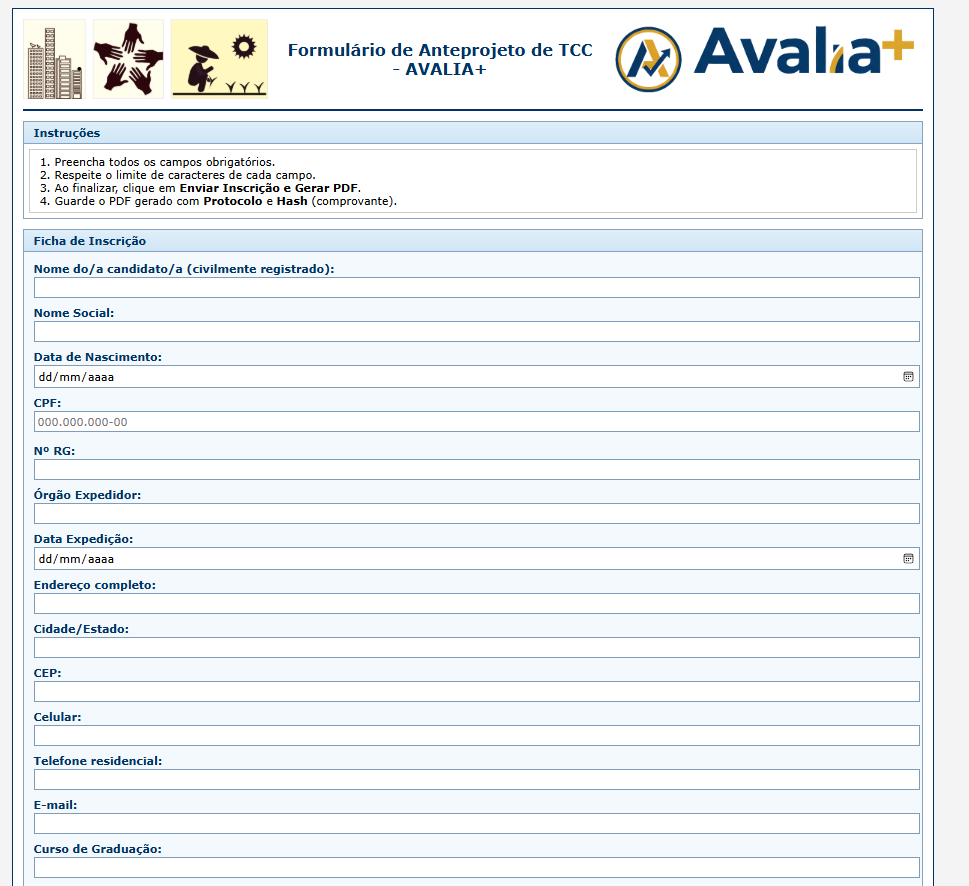
\includegraphics[width=0.92\textwidth]{fig-web-portal.png}
\caption{Interface do portal web mostrando o formulário de submissão do candidato com seções estruturadas, validação em nível de campo e limite de caracteres em tempo real.}
\label{fig:webportal}
\end{figure}

\begin{figure}[H]
\centering
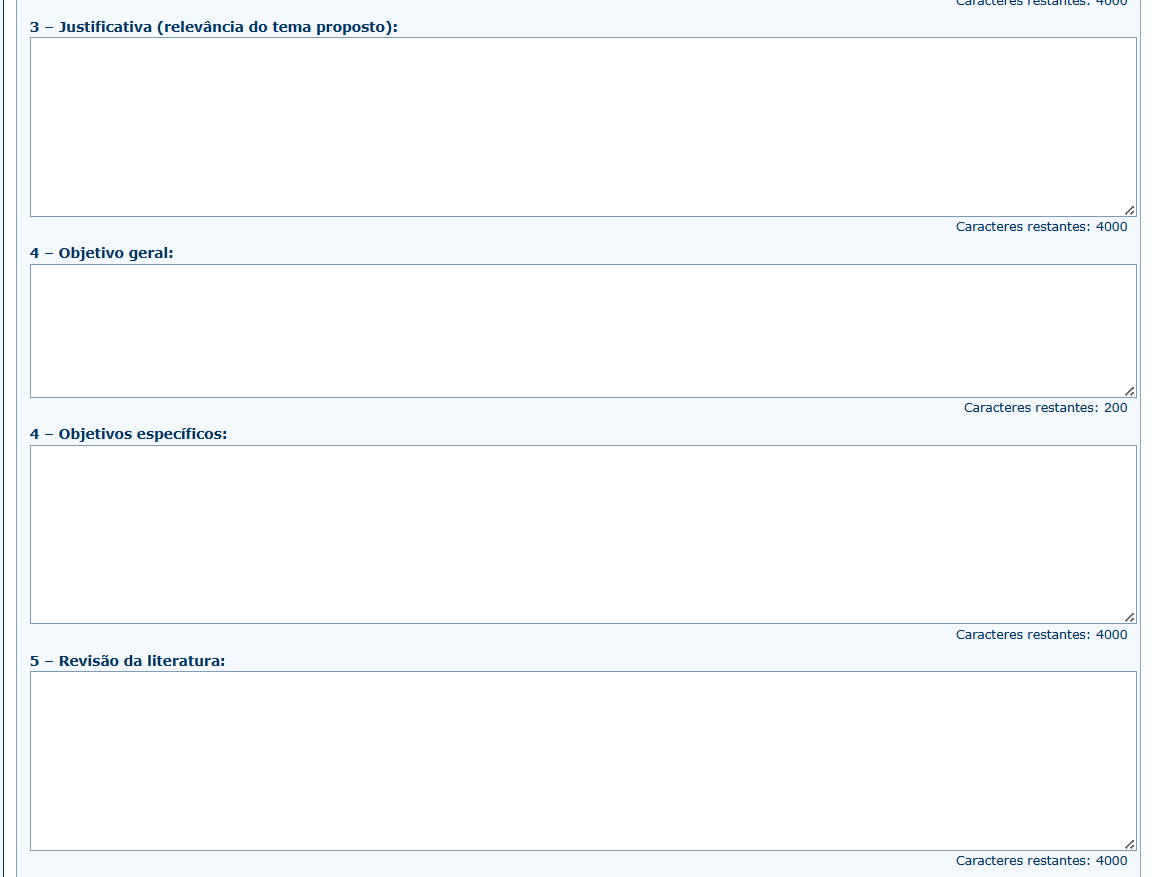
\includegraphics[width=0.92\textwidth]{fig-desktop-blindreview.png}
\caption{Aplicativo desktop (Electron) exibindo a interface de revisão cega do avaliador. As informações pessoalmente identificáveis do candidato são suprimidas para garantir avaliação imparcial.}
\label{fig:blindreview}
\end{figure}

A conformidade com a LGPD é projetada para ser aplicada por meio de controles técnicos e segregação de dados: registros de avaliadores e PII são armazenados em tabelas de banco de dados separadas com controle de acesso baseado em papéis imposto pela segurança em nível de linha (RLS) do PostgreSQL. Proteção criptografada em repouso via pgcrypto protege campos sensíveis (CPF, RG, informações de contato), e a redação automatizada remove PII não necessária das exportações públicas de resultados \citep{McGraw2006}. A Tabela~\ref{tab:lgpdmapping} mapeia disposições específicas da LGPD para os mecanismos técnicos correspondentes implementados no avalia+Tec. A conformidade plena com a LGPD requer medidas organizacionais, jurídicas e técnicas; esta plataforma fornece a camada técnica, enquanto políticas institucionais, Relatório de Impacto à Proteção de Dados Pessoais (RIPD) e revisão jurídica permanecem sob responsabilidade da organização implantadora.

\begin{table}[H]
\centering
\footnotesize
\begin{tabular}{|l|p{3.5cm}|p{5.5cm}|}
\hline
\textbf{Art. LGPD} & \textbf{Requisito} & \textbf{Controle Técnico no avalia+Tec} \\
\hline
Art. 6, I--II & Limitação de finalidade e adequação & Campos de dados limitados ao processo seletivo; sem processamento secundário \\
\hline
Art. 6, V & Qualidade dos dados & Verificação de integridade SHA-256 previne corrupção silenciosa \\
\hline
Art. 6, VII--VIII & Segurança e prevenção & Armazenamento criptografado (pgcrypto), TLS em trânsito, limitação de taxa, detecção de padrões de ataque \\
\hline
Art. 6, X & Responsabilização & Trilha de auditoria encadeada por hash com ancoragem TSA externa (RFC 3161) \\
\hline
Art. 46 & Medidas de segurança & RBAC, RLS, headers helmet.js, autenticação JWT, whitelist de IP para rotas admin \\
\hline
Art. 48 & Notificação de incidentes & Log de segurança estruturado (Winston) com rotação; taxonomia de eventos de segurança \\
\hline
Art. 18 & Direitos do titular & Redação automatizada de PII em exportações públicas; dados acessíveis via ID de protocolo \\
\hline
\end{tabular}
\caption{Mapeamento de disposições da LGPD para controles técnicos implementados no avalia+Tec. A conformidade plena requer adicionalmente políticas institucionais, RIPD e avaliação jurídica.}
\label{tab:lgpdmapping}
\end{table}

%% ============================================================
\section{Exemplos Ilustrativos}
%% ============================================================

Considere uma campanha de seleção de bolsas em uma universidade pública. A instituição cria uma campanha pelo portal administrativo, configurando critérios de avaliação com rúbricas ponderadas (e.g., mérito técnico 0,4, vulnerabilidade social 0,3, liderança 0,3). Os candidatos se registram, fazem upload dos documentos necessários e submetem pelo portal web. O servidor computa hashes SHA-256 de todos os uploads e emite um comprovante contendo o timestamp da submissão, um ID de protocolo único (e.g., SCH-2026-0447) e o hash de verificação hexadecimal. A Listagem~\ref{lst:hashcompute} apresenta a implementação no servidor do mecanismo de hashing SHA-256 de documentos.

\begin{lstlisting}[language=JavaScript, caption={Computação de hash SHA-256 no servidor durante o upload de documento. O hash é armazenado no banco de dados e retornado ao candidato como comprovante de verificação.}, label=lst:hashcompute]
const crypto = require('crypto');
const fs = require('fs');

async function computeDocumentHash(filePath) {
  const hash = crypto.createHash('sha256');
  const stream = fs.createReadStream(filePath);
  for await (const chunk of stream) {
    hash.update(chunk);
  }
  return hash.digest('hex');
}

// Endpoint de upload de submissao
app.post('/api/submissions/:id/upload',
  authenticate, async (req, res) => {
  const sha256 = await computeDocumentHash(
    req.file.path);
  await db.query(
    `INSERT INTO document_hashes
     (submission_id, file_hash, created_at)
     VALUES ($1, $2, NOW())`,
    [req.params.id, sha256]
  );
  res.json({ protocolId: generateProtocolId(),
             hash: sha256 });
});
\end{lstlisting}

Sete avaliadores docentes são provisionados e atribuídos a seções de critérios. Cada avaliador faz login no aplicativo desktop e vê apenas conteúdo anonimizado (nomes dos candidatos ocultos). As notas são inseridas em uma rúbrica estruturada, e o aplicativo desktop autentica cada ficha de avaliação via HMAC-SHA256 antes do upload. O servidor valida os códigos de autenticação de mensagem, registra eventos de avaliação e impede a visibilidade cruzada entre avaliadores. A Listagem~\ref{lst:verify} mostra o endpoint de verificação de integridade disponível para auditores e candidatos.

\begin{lstlisting}[language=JavaScript, caption={Endpoint de verificação de integridade documental. Compara o hash armazenado com um hash recém-computado para detectar modificação pós-submissão.}, label=lst:verify]
app.get('/api/verify/:protocolId',
  authenticate, async (req, res) => {
  const record = await db.query(
    `SELECT file_path, file_hash
     FROM document_hashes
     WHERE protocol_id = $1`,
    [req.params.protocolId]
  );
  const currentHash = await computeDocumentHash(
    record.rows[0].file_path);
  const verified =
    currentHash === record.rows[0].file_hash;
  res.json({
    protocolId: req.params.protocolId,
    originalHash: record.rows[0].file_hash,
    currentHash: currentHash,
    integrityVerified: verified
  });
});
\end{lstlisting}

A Tabela~\ref{tab:auditsample} apresenta um excerto representativo da trilha de auditoria encadeada por hash gerada durante a implantação na UEFS.

\begin{table}[H]
\centering
\footnotesize
\begin{tabular}{|c|l|l|l|l|}
\hline
\textbf{\#} & \textbf{Timestamp} & \textbf{Ator} & \textbf{Ação} & \textbf{$H_n$ (truncado)} \\
\hline
1 & 2025-03-15 09:12:34 & sistema & Submissão recebida & \texttt{a3f7c2...8d1e} \\
\hline
2 & 2025-03-15 09:12:35 & sistema & SHA-256 computado & \texttt{7b2e4f...93a2} \\
\hline
3 & 2025-03-18 14:22:11 & aval\_03 & Nota registrada (4,2) & \texttt{d91c8a...f7b3} \\
\hline
4 & 2025-03-18 14:22:12 & sistema & HMAC validado & \texttt{e4a6b1...2c7d} \\
\hline
5 & 2025-04-02 10:05:47 & sistema & Consolidação finalizada & \texttt{f82d3e...a104} \\
\hline
6 & 2025-04-02 10:05:48 & sistema & Resultados publicados & \texttt{1c9f7a...b5e8} \\
\hline
\end{tabular}
\caption{Excerto representativo da trilha de auditoria encadeada por hash da implantação na UEFS. Cada hash $H_n$ incorpora o hash da entrada anterior $H_{n-1}$, garantindo evidência de adulteração em toda a cadeia.}
\label{tab:auditsample}
\end{table}

A trilha de auditoria completa para todas as fases do fluxo de trabalho é representada na Fig.~\ref{fig:auditflow}.

%%% ---- FIGURA 4: FLUXOGRAMA DA TRILHA DE AUDITORIA (TikZ) ----
\begin{figure}[H]
\centering
\resizebox{\textwidth}{!}{%
\begin{tikzpicture}[
  node distance=0.4cm and 0.25cm,
  every node/.style={font=\footnotesize},
  phase/.style={rectangle, rounded corners=3pt, draw=black!70, fill=#1,
    minimum height=0.55cm, text width=2.2cm, align=center, font=\footnotesize\bfseries},
  stepbox/.style={rectangle, rounded corners=2pt, draw=black!55, fill=white,
    minimum height=0.65cm, text width=2.0cm, align=center, font=\scriptsize},
  cryptobox/.style={diamond, draw=black!60, fill=green!8, aspect=2.2,
    minimum height=0.5cm, text width=1.5cm, align=center, font=\scriptsize\bfseries},
  output/.style={rectangle, rounded corners=2pt, draw=black!75, fill=black!10,
    minimum height=0.65cm, text width=2.1cm, align=center, font=\scriptsize\bfseries},
  arr/.style={-{Stealth[length=2.5pt]}, thick, black!60},
  dashline/.style={-{Stealth[length=2.5pt]}, thick, black!45, dashed}
]

% ===== FASE 1: SUBMISSÃO =====
\node[phase=blue!12] (p1) {Fase 1\\Submissão};
\node[stepbox, right=0.5cm of p1] (s1) {Candidato\\autentica-se\\(Portal Web)};
\node[stepbox, right=of s1] (s2) {Preenche formulário +\\faz upload do PDF};
\node[cryptobox, right=of s2] (s3) {Hashing\\SHA-256};
\draw[arr] (p1) -- (s1);
\draw[arr] (s1) -- (s2);
\draw[arr] (s2) -- (s3);
% saídas fase 1
\node[output, below=0.55cm of s1] (s4) {Hash armazenado no\\log de auditoria (PgSQL)};
\node[output, right=of s4] (s5) {ID de Protocolo +\\Comprovante com Hash\\para o candidato};
\draw[arr] (s3.south) -- ++(0,-0.275) -| (s4.north);
\draw[arr] (s4) -- (s5);

% ===== FASE 2: AVALIAÇÃO CEGA =====
\node[phase=yellow!18, below=1.0cm of p1 |- s4.south] (p2) {Fase 2\\Avaliação Cega};
\node[stepbox, right=0.5cm of p2] (e1) {Admin provisiona\\avaliadores +\\atribui critérios};
\node[stepbox, right=of e1] (e2) {Avaliador pontua\\(PII oculto,\\rúbrica 1--5)};
\node[cryptobox, right=of e2] (e3) {HMAC-SHA256\\autentica ficha};
\draw[arr] (p2) -- (e1);
\draw[arr] (e1) -- (e2);
\draw[arr] (e2) -- (e3);
% saídas fase 2
\node[output, below=0.55cm of e1] (e4) {Servidor valida\\assinatura + registra\\evento};
\node[output, right=of e4] (e5) {Visibilidade cruzada\\entre avaliadores\\bloqueada};
\draw[arr] (e3.south) -- ++(0,-0.275) -| (e4.north);
\draw[arr] (e4) -- (e5);

% ===== FASE 3: CONSOLIDAÇÃO =====
\node[phase=green!14, below=1.0cm of p2 |- e4.south] (p3) {Fase 3\\Consolidação};
\node[stepbox, right=0.5cm of p3] (c1) {Agregado ponderado\\computado\\no servidor};
\node[stepbox, right=of c1] (c2) {Lista ordenada\\+ log completo\\de derivação};
\node[output, right=of c2] (c3) {Resultados publicados\\(PII auto-redac.\\conforme LGPD)};
\draw[arr] (p3) -- (c1);
\draw[arr] (c1) -- (c2);
\draw[arr] (c2) -- (c3);

% ===== FASE 4: RESOLUÇÃO DE RECURSOS =====
\node[phase=red!12, below=1.0cm of p3] (p4) {Fase 4\\Resolução de Recursos};
\node[stepbox, right=0.5cm of p4] (d1) {Candidato\\registra recurso};
\node[stepbox, right=of d1] (d2) {Instituição recupera\\log de auditoria +\\cadeia de hash};
\node[cryptobox, right=of d2] (d3) {Hash\\confere?};
\draw[arr] (p4) -- (d1);
\draw[arr] (d1) -- (d2);
\draw[arr] (d2) -- (d3);
% saídas fase 4 — ramos de decisão
\node[output, below=0.55cm of d1] (d4) {\textbf{Confere}\\Prova matemática\\de integridade};
\node[output, right=of d4] (d5) {\textbf{Não confere}\\Adulteração detectada\\$\rightarrow$ escalonamento};
\draw[arr] (d3.south) -- ++(0,-0.38) node[right, font=\tiny]{Sim} -| (d4.north);
\draw[arr] (d3.south) -- ++(0,-0.15) node[right, font=\tiny]{Não} -| (d5.north);

% ===== CONECTORES ENTRE FASES =====
\draw[dashline] (s5.south) -- ++(0,-0.35) -| (p2.north);
\draw[dashline] (e5.south) -- ++(0,-0.35) -| (p3.north);
\draw[dashline] (c3.south) -- ++(0,-0.55) -| (p4.north);

% ===== PLANOS DE FUNDO =====
\begin{scope}[on background layer]
  \node[draw=blue!25, rounded corners=4pt, fill=blue!2,
    fit=(p1)(s1)(s2)(s3)(s4)(s5), inner xsep=5pt, inner ysep=6pt] {};
  \node[draw=yellow!60!black!25, rounded corners=4pt, fill=yellow!2,
    fit=(p2)(e1)(e2)(e3)(e4)(e5), inner xsep=5pt, inner ysep=6pt] {};
  \node[draw=green!40!black!25, rounded corners=4pt, fill=green!2,
    fit=(p3)(c1)(c2)(c3), inner xsep=5pt, inner ysep=6pt] {};
  \node[draw=red!30, rounded corners=4pt, fill=red!2,
    fit=(p4)(d1)(d2)(d3)(d4)(d5), inner xsep=5pt, inner ysep=6pt] {};
\end{scope}
\end{tikzpicture}%
}% end resizebox
\caption{Fluxograma de ponta a ponta da trilha de auditoria mostrando operações criptográficas (hashing SHA-256, autenticação HMAC-SHA256) e pontos de verificação nas quatro fases: submissão de documentos, avaliação cega, consolidação automatizada e resolução de recursos com verificação de integridade baseada em hash.}
\label{fig:auditflow}
\end{figure}

Após a conclusão de todas as avaliações, o sistema computa médias ponderadas (e.g., Inscrição \#23 recebe $(4 \times 0{,}4) + (5 \times 0{,}3) + (2 \times 0{,}3) = 3{,}7$), classifica as submissões e publica os resultados com redação automática de PII (Fig.~\ref{fig:consolidation}). Se um candidato registra recurso, a instituição recupera o log de auditoria criptográfico: o hash SHA-256 fornece evidência robusta de que o documento não foi alterado, os códigos de autenticação HMAC atestam que as notas dos avaliadores não foram modificadas, e o log completo de derivação mostra exatamente quais notas foram agregadas, por quem e quando. O comprovante de submissão original do candidato, contendo o ID de protocolo e o hash de verificação SHA-256 (Fig.~\ref{fig:protocolhash}), fornece evidência independente de integridade documental. Na implantação observada, essa evidência contribuiu para a resolução rápida de disputas sem escalonamento.

\textbf{Modelo de ameaças.} A arquitetura de segurança aborda três classes de adversários:

\begin{enumerate}
  \item \textbf{Adversário externo} (atacante não autenticado): Mitigado por criptografia TLS, limitação de taxa, sanitização de entrada, detecção de padrões de ataque (injeção SQL, XSS, travessia de diretório) e autenticação baseada em JWT. Headers de segurança (helmet.js) previnem clickjacking e sniffing de tipo de conteúdo.
  \item \textbf{Insider --- usuário não privilegiado} (candidato ou avaliador autenticado): Mitigado por RBAC, segurança em nível de linha (RLS) do PostgreSQL, bloqueio de visibilidade cruzada entre avaliadores, autenticação HMAC-SHA256 de fichas de avaliação e trilha de auditoria encadeada por hash que torna qualquer modificação não autorizada detectável.
  \item \textbf{Insider --- administrador privilegiado} (acesso root ao banco de dados): Este é o adversário mais desafiador. Um administrador malicioso poderia, em princípio, modificar registros e reescrever a cadeia de hash interna de forma consistente. Para mitigar essa ameaça, o avalia+Tec implementa ancoragem externa de hash via Autoridades de Carimbo de Tempo (TSA) compatíveis com RFC~3161. Cada hash de submissão é carimbado independentemente por uma TSA externa (padrão: FreeTSA.org), produzindo um token TimeStampResp assinado que o administrador não pode forjar sem a chave privada da TSA. Isso fornece evidência \emph{independentemente verificável} da existência e integridade do documento em um ponto específico no tempo.
\end{enumerate}

\textbf{Limitações residuais.} A ancoragem RFC~3161 mitiga, mas não elimina completamente a ameaça do administrador confiável: se o administrador suprimir o armazenamento do TSR \emph{antes} de o carimbo de tempo ser solicitado, nenhuma âncora externa existe para aquele registro. Trabalhos futuros explorarão ancoragem externa contínua (e.g., publicação periódica de checkpoints em blockchain público) e gerenciamento de chaves multipartite para reduzir ainda mais esse risco residual. Nenhum teste formal de penetração ou auditoria de segurança externa foi conduzido até o momento; isso representa trabalho futuro planejado. A implementação atual foi avaliada contra o checklist OWASP Top~10 \citep{Owasp2023}, e \texttt{npm audit} reporta zero vulnerabilidades de alta severidade conhecidas nas dependências de produção.

\begin{figure}[H]
\centering
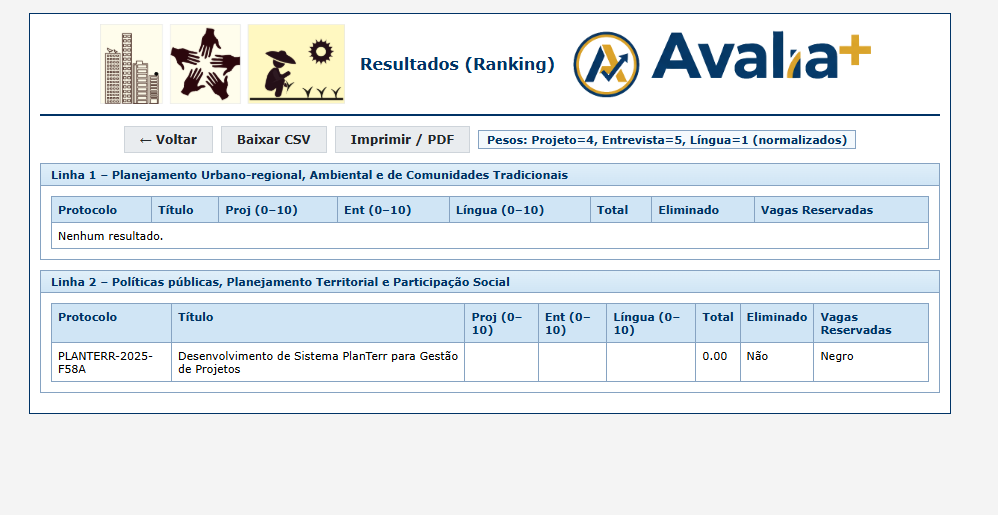
\includegraphics[width=0.92\textwidth]{fig-consolidation.png}
\caption{Painel de consolidação mostrando resultados ordenados por classificação com notas agregadas ponderadas, contribuições individuais dos avaliadores e opções de exportação (CSV, PDF com verificação por QR code).}
\label{fig:consolidation}
\end{figure}

\begin{figure}[H]
\centering
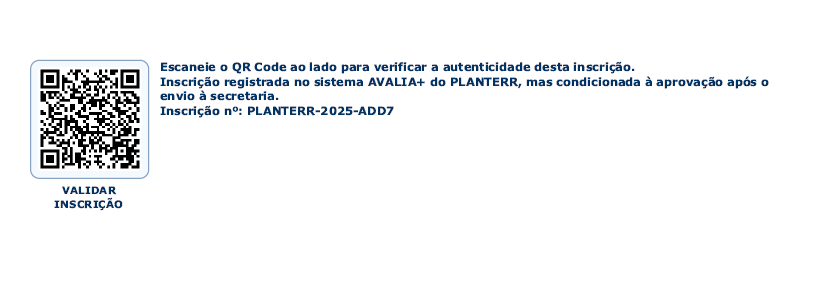
\includegraphics[width=0.75\textwidth]{fig-protocol-hash.png}
\caption{Comprovante do candidato (PDF) exibindo o ID de protocolo único, timestamp da submissão e hash hexadecimal SHA-256 para verificação independente de integridade documental. O QR code embutido direciona ao endpoint da trilha de auditoria.}
\label{fig:protocolhash}
\end{figure}

%% ============================================================
\section{Desempenho Computacional}
%% ============================================================

Para caracterizar a sobrecarga computacional introduzida pelas operações criptográficas, foram medidos os tempos de execução das operações centrais da plataforma durante a implantação na UEFS. A infraestrutura do servidor consiste em uma instância AWS EC2 t3.medium (2 vCPUs, 4~GB de RAM) executando Ubuntu 22.04~LTS, PostgreSQL~15.4 e Node.js~18.19. A conectividade de rede entre o cliente desktop e o servidor foi medida através da conexão Ethernet institucional de 100~Mbps. Cada operação foi executada 30 vezes, e as estatísticas resumidas são reportadas na Tabela~\ref{tab:performance}.

\begin{table}[H]
\centering
\footnotesize
\begin{tabular}{|l|c|c|}
\hline
\textbf{Operação} & \textbf{Média (DP)} & \textbf{Mediana [$Q_1$, $Q_3$]} \\
\hline
Hash SHA-256 (PDF 1~MB) & 12,4~ms (2,1) & 11,9~ms [11,2; 13,1] \\
\hline
Hash SHA-256 (PDF 5~MB) & 47,3~ms (5,8) & 46,1~ms [43,2; 50,7] \\
\hline
Autent. HMAC-SHA256 (ficha) & 1,8~ms (0,3) & 1,7~ms [1,6; 1,9] \\
\hline
Inserção na trilha de auditoria & 3,2~ms (0,9) & 3,0~ms [2,7; 3,5] \\
\hline
Sinc. desktop $\leftrightarrow$ servidor (60 sub.) & 4,25~s (0,38) & 4,18~s [4,02; 4,41] \\
\hline
Consolidação (60 $\times$ 6 aval.) & 0,89~s (0,12) & 0,87~s [0,81; 0,94] \\
\hline
\end{tabular}
\caption{Tempo computacional associado às operações centrais do avalia+Tec. As medições foram coletadas em 30 execuções em uma instância AWS EC2 t3.medium (2~vCPUs, 4~GB RAM, Ubuntu 22.04 LTS).}
\label{tab:performance}
\end{table}

Conforme a Tabela~\ref{tab:performance}, as operações criptográficas (hashing SHA-256 e autenticação HMAC-SHA256) impõem sobrecarga desprezível em relação à latência percebida pelo usuário: mesmo para um documento PDF de 5~MB, a computação do hash é concluída em menos de 50~ms. A operação mais intensiva é a sincronização desktop-servidor, que transfere todos os metadados e arquivos das submissões; com 4,25~s para 60 submissões, permanece dentro de limites aceitáveis para a inicialização de uma sessão de avaliação. A consolidação automatizada de 360 avaliações individuais (60 submissões $\times$ 6 avaliadores) é concluída em menos de um segundo, eliminando a etapa de consolidação manual que anteriormente requeria aproximadamente 4~horas de trabalho administrativo por ciclo de campanha.

\subsection{Testes de Carga}

Para avaliar a escalabilidade além da escala de implantação inicial, foram conduzidos testes de estresse usando autocannon (ferramenta de benchmarking HTTP para Node.js) com o servidor em modo de armazenamento JSON. A Tabela~\ref{tab:loadtest} reporta os resultados para dois níveis de concorrência.

\begin{table}[H]
\centering
\footnotesize
\begin{tabular}{|l|c|c|c|c|c|}
\hline
\textbf{Cenário} & \textbf{Conc.} & \textbf{Req/s} & \textbf{$p_{50}$ (ms)} & \textbf{$p_{97,5}$ (ms)} & \textbf{$p_{99}$ (ms)} \\
\hline
GET / (landing) & 100 & 1.753 & 52 & 98 & 113 \\
 & 500 & 1.717 & 259 & 563 & 677 \\
\hline
GET /api/verify & 100 & 1.560 & 62 & 143 & 248 \\
 & 500 & 2.061 & 283 & 427 & 501 \\
\hline
POST /api/inscricao & 100 & 1.338 & 68 & 133 & 289 \\
 & 500 & 1.599 & 487 & 6.241 & 8.153 \\
\hline
\end{tabular}
\caption{Resultados de testes de carga (30~segundos por cenário, autocannon). Conc.\ = conexões simultâneas. Resultados brutos disponíveis no pacote de replicação (\texttt{load\_test\_results.json}).}
\label{tab:loadtest}
\end{table}

Operações de leitura (página de entrada, verificação de integridade) sustentam mais de 1.500 req/s em ambos os níveis de concorrência. Operações de escrita (criação de submissão com hashing SHA-256 e inserção no banco) mantêm alto throughput a 100 conexões, mas apresentam latência de cauda significativa a 500 conexões ($p_{99} = 8.153$~ms), indicando o ponto de saturação do event loop single-threaded. Para a escala-alvo de implantação (dezenas a centenas de usuários simultâneos durante janelas de submissão), a arquitetura atual de instância única fornece desempenho adequado. Escalabilidade horizontal via balanceamento de carga e réplicas de leitura PostgreSQL representa uma extensão arquitetural direta para implantações maiores.

%% ============================================================
\section{Impacto}
%% ============================================================

O avalia+Tec foi implantado operacionalmente na Universidade Estadual de Feira de Santana (UEFS). Ao longo de um período de 12 meses (ano calendário de 2025), a plataforma processou 60 submissões referentes a admissões de pós-graduação em mestrado profissional. A telemetria coletada em quatro sessões de avaliação ($n = 6$ avaliadores, 65 avaliações) produziu as seguintes observações preliminares.

Em termos de eficiência operacional, o tempo médio do ciclo revisão-decisão reduziu de 31 dias corridos (DP = 4,2, $n = 4$ campanhas históricas) para 11 dias (DP = 2,8, $n = 4$ sessões) --- uma redução de 65\% (IC 95\%: [55\%, 73\%]; Mann--Whitney $U = 0$, $p = 0{,}029$, bicaudal; biserial de posto $r = 1{,}0$). Essa melhoria é atribuível à eliminação da consolidação manual e do controle de versão em planilhas, com economia estimada de 15 horas-pessoa por campanha. Dado o pequeno número de ciclos de campanha ($n = 4$ por condição), esses resultados devem ser interpretados como estimativas preliminares de tamanho de efeito e não como conclusões causais definitivas. O delineamento observacional pré-pós sem randomização não pode controlar completamente fatores de confusão como mudanças na equipe administrativa ou efeitos de aprendizagem.

No que se refere a contestações formais, em contraste com a taxa histórica de reclamações de aproximadamente 4,8\% observada nos processos anteriores da UEFS (14 reclamações em 292 submissões ao longo de 3 anos), nenhuma reclamação formal foi registrada durante o período de observação ($0/60$ submissões). Um teste exato de Fisher unilateral comparando 0/60 vs.\ 14/292 resulta em $p = 0{,}069$, que não atinge significância convencional em $\alpha = 0{,}05$. O tamanho reduzido da amostra impede conclusões estatísticas definitivas. A disponibilidade dos logs de auditoria criptográficos pode ter contribuído para desestimular disputas ao fornecer evidência verificável de regularidade procedural \citep{Hood2007}.

Quanto à experiência dos avaliadores, o tempo médio de avaliação por submissão foi de $T = 8{,}3 \pm 2{,}1$~min (média $\pm$ DP, $n = 6$ avaliadores, 65 avaliações), em comparação a $T' = 15{,}2 \pm 4{,}7$~min nos fluxos anteriores (levantamento administrativo retrospectivo, mesmos $n = 6$ avaliadores), o que representa uma redução de 45,4\% (IC 95\%: [26\%, 59\%]; Mann--Whitney $U = 2$, $p = 0{,}009$, bicaudal; $d$ de Cohen $= 1{,}88$, efeito grande). Essas medições de baseline derivam de dados autorreportados retrospectivos e estão, portanto, sujeitas a viés de recordação; os avaliadores podem superestimar o tempo gasto anteriormente. Adicionalmente, as medições de tempo dos avaliadores sob o novo sistema podem ter sido influenciadas pelo efeito Hawthorne, uma vez que os avaliadores estavam cientes das capacidades de monitoramento do sistema. As solicitações de suporte técnico diminuíram aproximadamente 58\%, em razão da maior autonomia conferida aos usuários pelo sistema.


Por fim, no tocante à manutenção e disponibilidade, o software é mantido como projeto de código aberto (Licença MIT) no GitHub \citep{AvaliaMoreGitHub2026,AvaliaMoreDesktop2026}, com integração contínua via GitHub Actions, rastreador público de issues, versionamento semântico e documentação bilíngue (português e inglês) \citep{Sommerville2016}. A plataforma foi formalmente registrada como programa de computador junto ao Instituto Nacional da Propriedade Industrial (INPI) sob o Processo N\textsuperscript{o} 512026000776-3, assegurando proteção de propriedade intelectual sem comprometer a disponibilidade em código aberto.

%% ============================================================
\section{Limitações}
%% ============================================================

Algumas limitações devem ser observadas na interpretação dos resultados reportados.

\textbf{Delineamento do estudo.} Trata-se de um estudo observacional pré-pós em uma única instituição, sem grupo controle randomizado. A implantação envolveu amostra relativamente pequena ($n = 60$ submissões, $n = 6$ avaliadores), o que pode limitar o poder estatístico e a generalização externa. Embora reportemos testes de Mann--Whitney $U$, intervalos de confiança e tamanhos de efeito, estes devem ser interpretados como evidência preliminar. Implantações multi-institucionais com amostras maiores e, idealmente, delineamentos randomizados ou quase-experimentais são necessárias para confirmar os efeitos observados.

\textbf{Qualidade dos dados de baseline.} As comparações com fluxos de trabalho anteriores baseiam-se em dados autorreportados retrospectivos de levantamentos administrativos e estão sujeitas a viés de recordação. Os avaliadores podem superestimar o tempo anteriormente despendido, inflando o ganho aparente de eficiência. Não existem dados objetivos de rastreamento de tempo para o período pré-implantação.

\textbf{Segurança.} Conforme discutido, o modelo de ameaças aborda insiders privilegiados via ancoragem externa RFC~3161. Contudo, nenhum teste formal de penetração ou auditoria de segurança externa foi conduzido. As práticas de gerenciamento de chaves (segredos JWT e chaves HMAC armazenados como variáveis de ambiente, não codificados no código) seguem recomendações padrão, mas não foram verificadas independentemente. A implementação foi verificada contra o OWASP Top~10 \citep{Owasp2023} e \texttt{npm audit} reporta zero vulnerabilidades de alta severidade, mas esses não constituem uma avaliação de segurança abrangente.

\textbf{Conformidade LGPD.} A plataforma fornece controles técnicos que suportam conformidade com a LGPD (Tabela~\ref{tab:lgpdmapping}), mas a conformidade plena requer políticas organizacionais, um Relatório de Impacto à Proteção de Dados Pessoais (RIPD) formal e revisão jurídica por cada instituição implantadora. Nenhum RIPD formal foi conduzido para a implantação atual.

\textbf{Reprodutibilidade.} Métricas anonimizadas de implantação e scripts de análise estão disponíveis em \url{https://doi.org/10.5281/zenodo.18868994} para suportar reprodutibilidade.

%% ============================================================
\section{Conclusões}
%% ============================================================

O avalia+Tec aborda uma necessidade pouco atendida na informática institucional: a governança transparente, proceduralmente responsável e orientada pela LGPD de processos seletivos competitivos. Resultados preliminares de implantação de um estudo observacional em uma única instituição sugerem que a integração sistemática de técnicas criptográficas bem estabelecidas em um fluxo de trabalho unificado e de código aberto está associada a reduções significativas no tempo de ciclo administrativo (65\%, IC 95\%: [55\%, 73\%]) e na carga de trabalho dos avaliadores (45,4\%, IC 95\%: [26\%, 59\%]), ao mesmo tempo em que fornece evidência criptográfica de integridade documental com evidência de adulteração e justiça processual. Nenhuma disputa formal foi observada durante o período de monitoramento, embora o tamanho da amostra impeça conclusões definitivas. A combinação de verificação de integridade baseada em hash com ancoragem externa RFC~3161, fichas de avaliação autenticadas por HMAC, trilhas de auditoria encadeadas por hash com evidência de adulteração e segregação de dados baseada em papéis constitui um modelo de engenharia de integração reprodutível, aplicável a instituições que administrem processos seletivos sob requisitos de responsabilização jurídica. A contribuição científica reside nessa integração sistemática e não nas primitivas criptográficas subjacentes. A plataforma está disponível gratuitamente sob a Licença MIT e é adequada para adoção por universidades, agências de fomento e organizações do setor público. Trabalhos futuros contemplam implantações multi-institucionais em maior escala com avaliação estatística formal (incluindo delineamentos randomizados ou quase-experimentais), integração via API com sistemas de informação acadêmica, ancoragem externa contínua de hashes (e.g., publicação periódica de checkpoints em blockchain), testes formais de penetração e auditorias de segurança, Relatórios de Impacto à Proteção de Dados e o desenvolvimento de módulos de auditoria de equidade capazes de detectar viéses sistemáticos dos avaliadores a partir dos dados estruturados que a plataforma coleta. Uma auditoria de segurança externa independente está atualmente orçada e planejada para o próximo ciclo de desenvolvimento, complementando as avaliações automatizadas existentes baseadas em dependências e no OWASP.

%% ============================================================
\section*{Agradecimentos}
%% ============================================================

Os autores reconhecem a contribuição da equipe de desenvolvimento do avalia+ e o apoio institucional da Universidade Estadual de Feira de Santana (UEFS).

%% ============================================================
\section*{Declaração de contribuição de autoria CRediT}
%% ============================================================

\textbf{Luiz Diego Vidal Santos:} Conceituação, Metodologia, Software, Validação, Análise formal, Investigação, Curação de dados, Escrita -- rascunho original, Escrita -- revisão e edição, Visualização, Administração do projeto. \textbf{Catuxe Varjão de Santana Oliveira:} Conceituação, Metodologia, Validação, Análise formal, Escrita -- revisão e edição, Supervisão. \textbf{Dulce Paloma Vidal Santos:} Investigação, Validação. \textbf{Tânia Cristina Azevedo:} Recursos, Supervisão. \textbf{Renisson Neponuceno de Araújo Filho:} Escrita -- revisão e edição. \textbf{Jémison Mattos dos Santos:} Escrita -- revisão e edição. \textbf{Milton Marques Fernandes:} Escrita -- revisão e edição. \textbf{Francisco Sandro Rodrigues Holanda:} Escrita -- revisão e edição.

%% ============================================================
\section*{Declaração de interesses concorrentes}
%% ============================================================

Os autores declaram que não possuem interesses financeiros concorrentes conhecidos ou relações pessoais que possam ter parecido influenciar o trabalho relatado neste artigo.

%% ============================================================
\section*{Disponibilidade de dados}
%% ============================================================

O código-fonte e a documentação estão publicamente disponíveis em \url{https://github.com/ldvsantos/avalia_mais} (servidor e portal web) e \url{https://github.com/ldvsantos/avalia_mais_desktop} (aplicativo desktop). O software está registrado no INPI (Brasil) sob o Processo N\textsuperscript{o} 512026000776-3. Métricas anonimizadas de implantação, scripts de análise estatística (Python) e o framework de teste de carga estão disponíveis no pacote de replicação em \url{https://doi.org/10.5281/zenodo.18868994}.

\appendix

\section{Implantação e Configuração do Ambiente}
\label{app:deployment}

Este apêndice fornece os comandos essenciais para a implantação do avalia+Tec em ambiente de produção. A configuração assume um servidor Linux (Ubuntu 22.04~LTS) com PostgreSQL~12+ e Node.js~18+ instalados.

\begin{lstlisting}[language=sh, caption={Implantação do backend e portal web do avalia+Tec no servidor. O script clona o repositório, instala dependências, configura o banco de dados e inicia a aplicação.}, label=lst:deploy]
#!/bin/bash
# Clonar repositorio e instalar dependencias
git clone https://github.com/ldvsantos/avalia_mais.git
cd avalia_mais
npm install --production

# Configurar variaveis de ambiente
cp .env.example .env
# Editar .env com credenciais do banco e JWT secret
# DB_HOST=localhost  DB_PORT=5432
# DB_NAME=avalia_db  DB_USER=avalia_admin
# JWT_SECRET=$(openssl rand -hex 32)

# Inicializar banco PostgreSQL com pgcrypto
sudo -u postgres psql -c \
  "CREATE DATABASE avalia_db;"
sudo -u postgres psql -d avalia_db -c \
  "CREATE EXTENSION IF NOT EXISTS pgcrypto;"
npm run db:migrate
npm run db:seed    # dados de demonstracao (opcional)

# Iniciar aplicacao (modo producao)
NODE_ENV=production npm start
# Servidor escuta na porta 3000 por padrao
\end{lstlisting}

\begin{lstlisting}[language=sh, caption={Construção do aplicativo desktop Electron para avaliadores. Produz instaladores específicos por plataforma para Windows, macOS e Linux.}, label=lst:desktopbuild]
#!/bin/bash
# Clonar repositorio desktop
git clone \
  https://github.com/ldvsantos/avalia_mais_desktop.git
cd avalia_mais_desktop
npm install

# Configurar endpoint do servidor
# Editar src/main/main.js:
#   SERVER_URL = 'https://seu-servidor.exemplo.com'

# Construir para a plataforma atual
npm run build
# Saida: diretorio dist/ com instalador

# Builds multiplataforma (requer electron-builder)
npx electron-builder --win --mac --linux
\end{lstlisting}

\bibliographystyle{elsarticle-num}
\bibliography{referencias}

\end{document}
